\chapter{Introduction}
For almost 4 billion years, single celled organisms dominated the planet.  About 650 million years ago, the first multicellular animals emerged in the ocean.  340 million years ago, amphibians escaped the ocean and walked on land.  About 6 million years ago, humans split away from chimps.  About 10,000 years ago, after the ice caps of the Pleistocene retreated, we began to develop agriculture.  The efficiency compared to hunting and gathering allowed for some people to live off the surplus of production, and not be wholly concerned with the daily grind.  This freed the human mind to do other things.  About 600 years ago, the Gutenberg Press was invented, allowing for broad dissemination of information.  In 1946, a giant room sized computer called the ENIAC consumed 174 kilowatts to compute 5000 additions per second.  The latest iPhone today can compute 10 trillion operations per second in your pocket.  

There are a wide range of estimates for how many operations per second a human brain effectively computes, but we are already seeing superhuman performance emerging for many tasks.  In 1997 IBM's Deep Blue beat Garry Kasparov the world chess champion.  In 2016, neural nets could classify images of skin cancer better than highly trained dermatologists.  Regardless of your stance on general AI, the most powerful computer known in the universe, the human mind, is being challenged.  But it is not really a challenge.  Eventually computers will outperform humans at every task.  Whether a computer has general intelligence will become a fuzzy question.  Pick a task, define a metric, gather enough data, apply gradient descent, and eventually a neural net will achieve superhuman performance.  No laws of physics prevent this.  It is arrogant to think that the human mind is something so magical a computer cannot surpass it.  The mind was developed to allow an organism to out-compete its neighbors at finding food and mates.  In the process, things like hunger, happiness, anger, memory, and wisdom, were all developed to maximize that organism's number of living descendants, while dealing with the obstacles on Earth.  I would argue the human mind is actually a very narrow intelligence developed to deal with Earthly animal problems.  A silicon based intelligence could very well be more general than narrow human intelligence.

\section{What is AI?}
At its heart, modern AI is actually very simple.  There are inputs, outputs, labels, and knobs (parameters).  The knobs control how the neural net produces an output given its input.  GPT3 has 175 billion knobs \cite{brown2020language}.  Training a neural net is tuning the knobs until you are happy with the outputs.  For example, imagine you want to train a neural net to predict whether an image is a cat or a dog.  The input would be an image.  To a neural net, an image is represented by a 2D array of pixels, and each pixel is represented by 3 numbers, corresponding to red, green, and blue intensities.  The output would be the probability that the picture is a cat (from which the probability for dog can be inferred).  The knobs are initially in random positions.  When the first image is passed through the neural net, it will likely output 50\%, since it does not know anything yet.  Say the picture is labelled as a cat.  The knobs must now be turned very slightly so that the net would have output a higher percentage for cat, maybe 51\% cat.  The amount a knob should turn can be determined by looking at how much the probability for cat changes given how much you turn that knob, holding all other knobs still.  This is called gradient descent. 
To train a neural net, continue passing labeled inputs and turning the knobs until the outputs are correct to your satisfaction.  It could be the case that you run out of data before the outputs are correct enough.  Then you can pass the dataset in again.  You can do this many times, but be careful because eventually the neural net will overfit to your training data, and will not generalize well to new inputs.  Periodically evaluating performance on a held out validation set is a good way to determine if the net has overfit on the training data yet.

The same concept can be used to train a neural net that generates text.  Again, there are inputs, outputs, labels, and knobs.  The input would be a sequence of words or characters.  To a neural net this is represented as a vector of zeros with a one at the index of that word or character in the dictionary.  The output would be the next word in the sequence.  This simple concept of inputs, outputs, labels, and tuning knobs with gradient descent is at the heart of the latest AI renaissance.

\section{A Longer Answer}

In 1943, a mathematician and a neurophysiologist published the first computational model of the neuron \cite{mcculloch1943logical}.  In 1958, the perceptron was invented \cite{rosenblatt1958perceptron}, which led to the multilayer perceptron a few years later.  In 1959 at Stanford, Bernard Widrow applied the first neural network to a real world problem, reducing noise in a phone line.  I was actually fortunate enough to attend a talk he gave here a few years ago, where he demonstrated the neural net he trained before even my parents were born.  Backpropagation as we know it today is widely credited to work by Hinton and others in 1986 \cite{rumelhart1986learning}, although the technique was already known in the 1960s as automatic differentiation \cite{wengert1964simple}.  The technique has been rediscovered many times.  After all, it is simply applying the derivative chain rule to a directed acyclic graph.  Powerful but simple, very much in the spirit of modern AI.  In 1989, Yann Lecun trained a convolutional neural network to recognize handwritten zip codes on mail \cite{lecun1989backpropagation}. ``LeNet", as he named it, took 3 days to train.  He later released an open dataset of handwritten digits called MNIST, which is still very popular.  This dataset contains 70,000 grayscale images, each of size 28x28 pixels, and takes up about 54MB of space total. 

In 2009, Fei-Fei Li's group at Stanford released ImageNet \cite{deng2009imagenet}.  The size of this dataset, about 150GB, was unprecedented.  When first released, the dataset included over 1 million labeled color images of every day objects such as cats and dogs.  The images varied in size. Resizing to about 256x256 was common practice.  There was no chance of fitting the dataset into memory back then, so people had to get pretty creative with low level logic, coordinating data across the hard drive, CPU memory, and GPU memory.  Knowledge of how to put together a computer from parts became highly valuable for a grad student, as every stat could be optimized for better AI performance.  For example, CPUs that supported a high number of PCIe lanes were highly sought after as GPUs use these to communicate, and the more the better.  I remember when an admin asked me for the receipt of my computer for reimbursement, and I had to get about 15 for all the different parts I purchased and assembled.  

Imagenet gave rise to Alex Krizhevsky's historical AlexNet \cite{krizhevsky2012imagenet}, dominating the ILSVRC 2012 competition and reigniting excitement in AI.  The AI winter was over.  Interestingly, AlexNet looks very similar to LeNet from 26 years prior, but much much bigger.  LeNet had about 60 thousand parameters and AlexNet had about 60 million.  AlexNet was 1000x bigger, and consumed about 100,000x as much compute.  See Figure \ref{fig:intro_ai_moores}.  AlexNet achieved a top-5 test error of about 16\%.  The next closest competitor had a 26\% error rate using hand-crafted SIFT features.  Human performance on ImageNet was determined to be about 5.1\% error.  This was surpassed in 2015 \cite{he2015delving} with a net that used parametric rectified linear unit activations.  For context, rectified linear units, $\max(0, x)$, became more favorable than sigmoid activations for whatever reason, who knows with neural nets really, and this parametric tweak increased performance.  A year later, that same researcher invented ResNets \cite{he2016deep}, introducing the skip connection.  These skip connections allow data and gradients to flow unimpeded by the layers, allowing for deeper networks to be trained more aggressively.  This contribution seems to have made more impact.

In 2012 it took 6 days on 2 GPUs to train AlexNet to 16\% top-5 error.  In April 2018, Google trained a 50 layer ResNet using a ``pod" of ``tensor processing units" to 7\% top-5 error in only 30 minutes.  As of the writing of this thesis, the fastest training of ImageNet to 7\% top-5 error rate is 2 minutes and 38 seconds, also using a 50 layer ResNet.  Stanford DawnBench \cite{coleman2017dawnbench}, maintained by Chris Re and his group, tracks this metric with an online leaderboard and all submissions are open source.

While the computer vision revolution was taking most of the headlines, natural language processing was moving less quickly.  But the progress in the last few years has been explosive.  Neural nets in NLP are getting so powerful and general that now they are even achieving state of the art results in computer vision.

In 2017 the NIPS paper ``Attention is All You Need" introduced the transformer model \cite{vaswani2017attention}.  While they are used for sequential data, transformers do not require the data to be processed in order. This allows for significantly more parallelization than RNNs (e.g. LSTMs \cite{hochreiter1997long}) and reduces training times.  With a transformer, the ``attention" paid to each element in a sequence is determined during the feed forward pass, with the ``attention" manifesting itself as a weighted sum.

Google published a transformer model called BERT in 2018 \cite{devlin2018bert} and achieved state of the art performance on a wide range of natural language processing tasks.  Every year OpenAI has been releasing a more powerful transformer model: GPT1 in 2018 \cite{radford2018improving}, GPT2 in 2019 \cite{radford2019language}, and GPT3 in 2020 \cite{brown2020language}.  GPT3 is arguably the most powerful neural net in the world.  At least that is known to the public.  Its 175 billion parameters consumed 314 zettaflops to train on 45 terabytes of text scraped from the internet.

A transformer model can be trained in an unsupervised manner.  Simply feed it a sequence with a subset of the sequence missing and ask it to predict the missing subset.  Once the model is trained, it can be used for sequence generation, sequence completion, choosing among a multiple choice set of sequences, and more.  These models can be used for all sorts of tasks.  If the task can be framed as a sequence to sequence problem, a transformer can be used.  For example, seed it with the sequence ``Q: What color is the sky? A: ".  Completing the sequence might give something like ``blue" or ``The sky is blue".  If only a finite set of options are valid, look at the score it gives to each option and pick the one with the highest score.  If the net is well trained, it will give higher weight to ``blue" than to ``red".  Notice that this makes the assumption that the net will understand what is meant by putting a ``Q:" in front of one sentence and then following it with an ``A:".  These transformer models do seem to just get it, and have some level of common sense.

GPT stands for Generative Pre-Trained Transformer, but it might as well stand for General Purpose Transformer, because that is how it is being used.  OpenAI showed that transformers are domain agnostic and can even be used for images as shown with ImageGPT \cite{chen2020generative}.  They argue that any type of data is a sequence on some level since all data can be represented as a sequence of bits.  Therefore a transformer model could be used in any domain.  ImageGPT achieved state of the art performance on CIFAR-10, outperforming the best ResNet, and showed competitive performance on ImageNet, but not yet state of the art.

In 2021, OpenAI released DALL-E \cite{ramesh2021zero}.  They adapted GPT2 to generate images from a sequence of text.  For example if the net is fed ``an armchair in the shape of an avocado", it will generate some very plausible images of what an avocado shaped armchair would look like.  There is a strong case to be made that a general architecture, maybe the transformer, can achieve state of the art results across all domains.  One net to rule them all. \\

\begin{figure}[h]
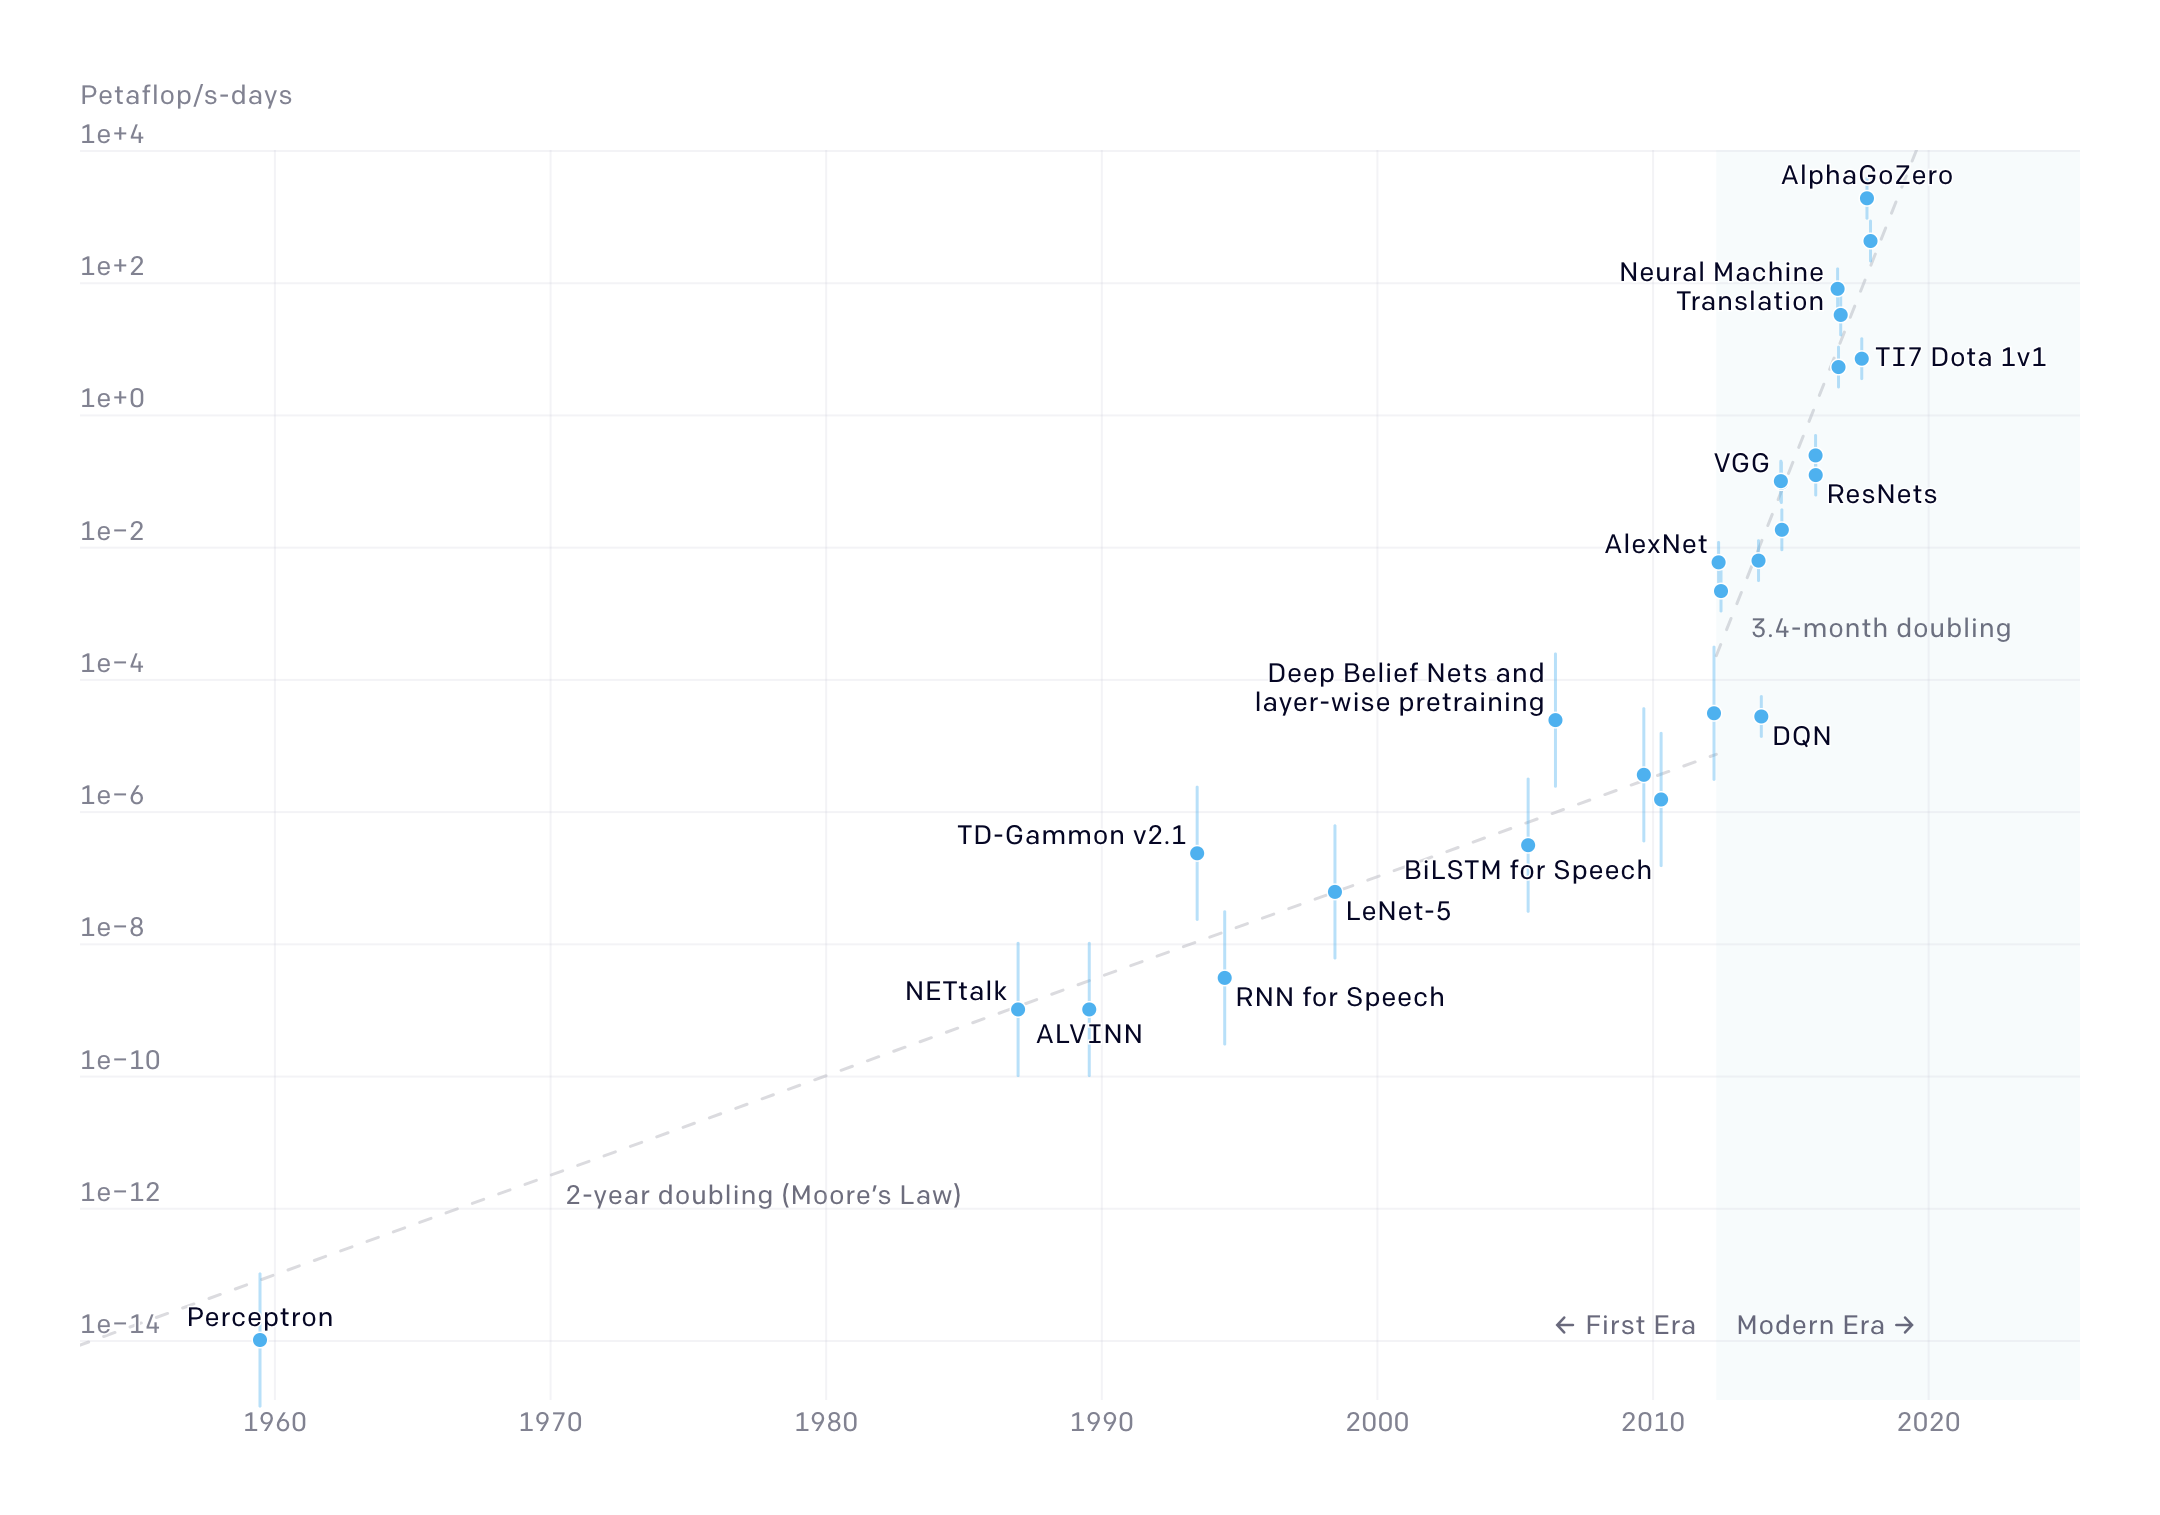
\includegraphics[width=\textwidth]{intro_ai_moores}
\caption{Exponential Growth of AI Compute}
\vspace{12px}
The modern AI era has seen a doubling in compute every 3.4 months.  This plot is already outdated.  GPT3 presented in June 2020 consumed 3.6e+5 petaflop-days of compute, which would be off the chart.  GPT3 consumed over 6 million times as much compute as AlexNet did in 2012, which was bleeding edge when I came to Stanford.  In fact, AlexNet was released the same month that I started graduate school.  Credit to OpenAI for the figure \cite{openai2018compute}.
\vspace{12px}
\label{fig:intro_ai_moores}
\end{figure}